%!Tex Root = ../Tutorat3.tex
% ./Packete.tex
% ./Design.tex
% ./Deklarationen.tex
% ./Aufgabe1.tex
% ./Aufgabe3.tex
% ./Aufgabe4.tex
% ./Bonus.tex

\section{Task 2}

\setcounter{task}{1}

\begin{frame}{Task 2}{Latest Deadline First}
  \begin{requirements}
    \begin{itemize}
      \item is \alert{non-preemptive}
      \item \alert{synchronous task activations}
      \item $min(D_i)$ for all remaning tasks $J_i$ \alert{without successors} or \alert{whose successors} have been all selected in the \alert{precedence graph}
        % select the tasks with the \alert{latest deadline} to be scheduled last.
      \item \alert{minimizes} the \alert{maximum lateness}
    \end{itemize}
  \end{requirements}
\end{frame}

\begin{frame}{Task 2}{Latest Deadline First}
  \centering
  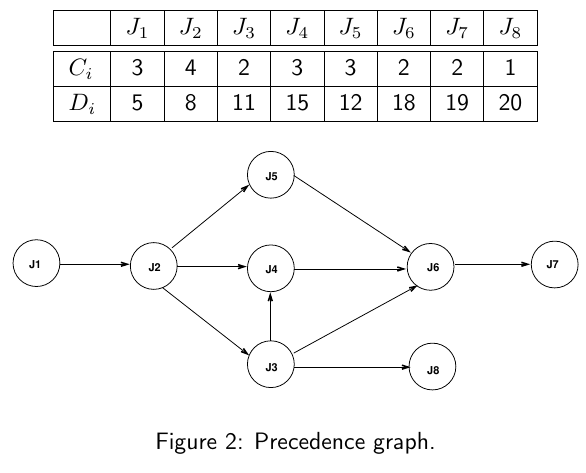
\includegraphics[height=0.7\paperheight]{./figures/2_tab_graph.png}
\end{frame}

\begin{frame}{Task 2}{Latest Deadline First}
  \centering
  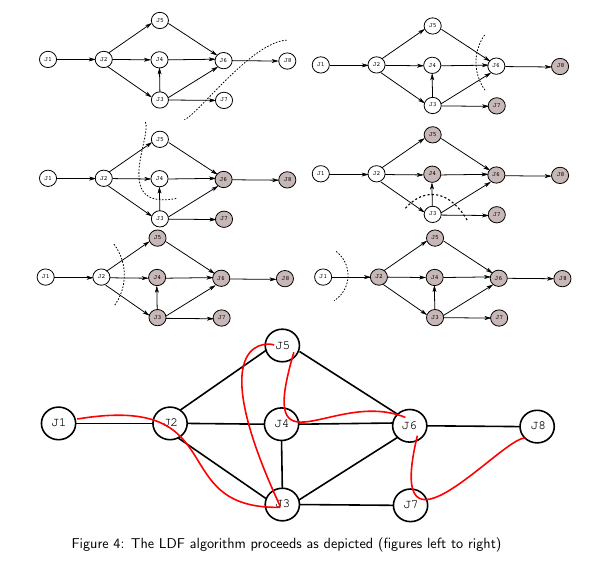
\includegraphics[height=0.7\paperheight]{./figures/2_steps.png}
\end{frame}

\begin{frame}{Task 2}{Latest Deadline First}
  \begin{itemize}
    \item \alert{queue of tasks:} (\qquad,\qquad,\qquad,\qquad,\qquad,\qquad,\qquad,\qquad)
  \end{itemize}
  \centering
  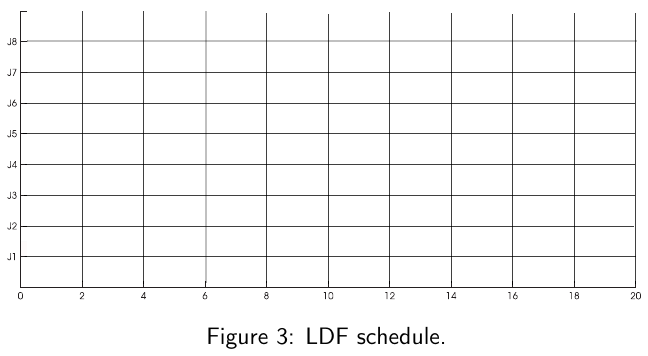
\includegraphics[width=0.7\textwidth]{./figures/2_empty.png}
\end{frame}

\begin{frame}{Task 2}{Latest Deadline First}
  \begin{itemize}
    \item \alert{queue of tasks:}  $(J_1, J_2, J_3, J_5, J_4, J_6, J_7, J_8)$
  \end{itemize}
  \centering
  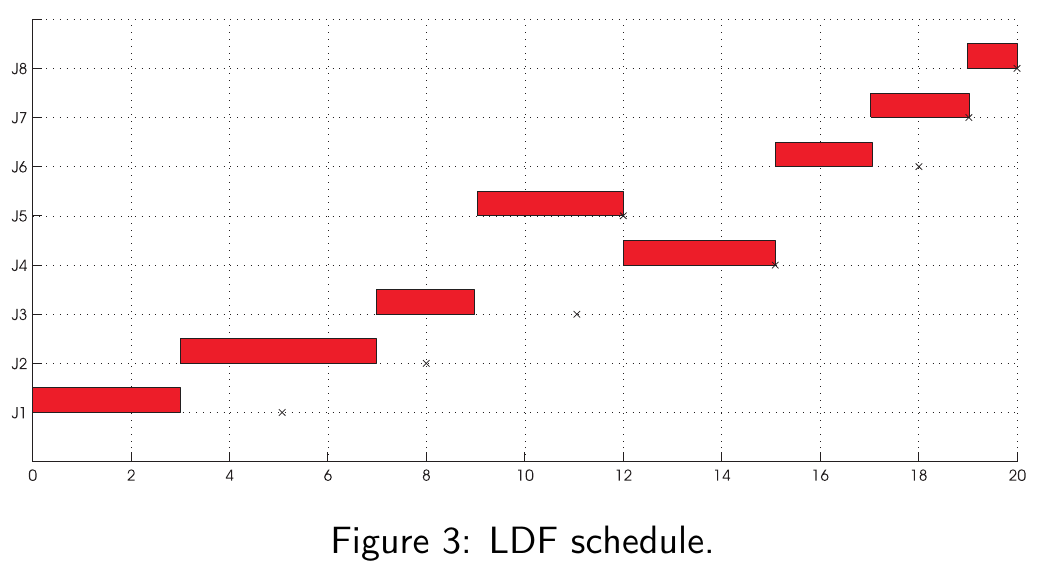
\includegraphics[width=0.7\textwidth]{./figures/2_sol.png}
\end{frame}
